% Options for packages loaded elsewhere
\PassOptionsToPackage{unicode}{hyperref}
\PassOptionsToPackage{hyphens}{url}
%
\documentclass[
]{article}
\usepackage{amsmath,amssymb}
\usepackage{iftex}
\ifPDFTeX
  \usepackage[T1]{fontenc}
  \usepackage[utf8]{inputenc}
  \usepackage{textcomp} % provide euro and other symbols
\else % if luatex or xetex
  \usepackage{unicode-math} % this also loads fontspec
  \defaultfontfeatures{Scale=MatchLowercase}
  \defaultfontfeatures[\rmfamily]{Ligatures=TeX,Scale=1}
\fi
\usepackage{lmodern}
\ifPDFTeX\else
  % xetex/luatex font selection
\fi
% Use upquote if available, for straight quotes in verbatim environments
\IfFileExists{upquote.sty}{\usepackage{upquote}}{}
\IfFileExists{microtype.sty}{% use microtype if available
  \usepackage[]{microtype}
  \UseMicrotypeSet[protrusion]{basicmath} % disable protrusion for tt fonts
}{}
\makeatletter
\@ifundefined{KOMAClassName}{% if non-KOMA class
  \IfFileExists{parskip.sty}{%
    \usepackage{parskip}
  }{% else
    \setlength{\parindent}{0pt}
    \setlength{\parskip}{6pt plus 2pt minus 1pt}}
}{% if KOMA class
  \KOMAoptions{parskip=half}}
\makeatother
\usepackage{xcolor}
\usepackage[margin=1in]{geometry}
\usepackage{graphicx}
\makeatletter
\def\maxwidth{\ifdim\Gin@nat@width>\linewidth\linewidth\else\Gin@nat@width\fi}
\def\maxheight{\ifdim\Gin@nat@height>\textheight\textheight\else\Gin@nat@height\fi}
\makeatother
% Scale images if necessary, so that they will not overflow the page
% margins by default, and it is still possible to overwrite the defaults
% using explicit options in \includegraphics[width, height, ...]{}
\setkeys{Gin}{width=\maxwidth,height=\maxheight,keepaspectratio}
% Set default figure placement to htbp
\makeatletter
\def\fps@figure{htbp}
\makeatother
\setlength{\emergencystretch}{3em} % prevent overfull lines
\providecommand{\tightlist}{%
  \setlength{\itemsep}{0pt}\setlength{\parskip}{0pt}}
\setcounter{secnumdepth}{-\maxdimen} % remove section numbering
\ifLuaTeX
  \usepackage{selnolig}  % disable illegal ligatures
\fi
\usepackage{bookmark}
\IfFileExists{xurl.sty}{\usepackage{xurl}}{} % add URL line breaks if available
\urlstyle{same}
\hypersetup{
  pdftitle={Breast Cancer Wisconsin Diagnostic Dataset},
  hidelinks,
  pdfcreator={LaTeX via pandoc}}

\title{Breast Cancer Wisconsin Diagnostic Dataset}
\author{}
\date{\vspace{-2.5em}}

\begin{document}
\maketitle

\subsection{Overview}\label{overview}

\begin{itemize}
\tightlist
\item
  \textbf{Description}: This project involved Exploratory Data Analysis
  (EDA) using the Breast Cancer Wisconsin (Diagnostic) dataset available
  from the
  \href{http://archive.ics.uci.edu/dataset/17/breast+cancer+wisconsin+diagnostic}{UC
  Irvine Machine Learning Repository}.
\end{itemize}

With only 569 cases and 30 features, the EDA processes included
Correlation Matrices, Linear Discriminant Analysis, Quadratic
Discriminant Analysis, Principal Component Analysis, and T-Distributed
Stochastic Neighbour Embedding.

The purpose of this project was to gain a basic understanding of which
variables are most important in determining whether cancer is malignant
or benign. To identify these key variables, two binary classification
models---Linear Discriminant Analysis (LDA) and Quadratic Discriminant
Analysis (QDA)---were employed.

To gain a more in-depth understanding of the importance of various
variables, Principal Component Analysis (PCA) and T-Distributed
Stochastic Neighbour Embedding (t-SNE) were utilised.

\subsection{Methodology}\label{methodology}

\begin{itemize}
\item
  \textbf{Technologies}: Various packages were used throughout this
  Exploratory Data Analysis of the Breast Cancer Wisconsin data,
  including \texttt{corrplot}, \texttt{readODS}, \texttt{dplyr},
  \texttt{tidyverse}, \texttt{MASS}, \texttt{ggplot2}, and
  \texttt{Rtsne}.
\item
  \textbf{Methods}: It is important to note that some columns from the
  original dataset were modified. The ID number was removed as it did
  not provide additional benefit to the EDA, and the diagnosis column
  was converted to a binary column, where malignant was classified as 1
  and benign as 0. This binary column is referred to as \texttt{cancer}
  in the modified dataframe. The \texttt{cancer} variable was the
  dependent variable for the EDA processes.
\end{itemize}

This project involved creating Correlation Matrices to recognise which
variables have the strongest correlations with others.

To perform LDA, the variables were scaled to have a mean of 0 and a
standard deviation of 1. The means and standard deviations of the scaled
variables were computed. For both LDA and QDA, the data was split into
70\% for training and 30\% for testing. The model was trained using the
70\% training dataset, with the \texttt{cancer} variable as the response
variable. This trained model was then tested using the 30\% testing
dataset, and the accuracy was calculated by comparing predicted versus
actual class labels.

QDA followed similar processes, with the exception that the variables
were not scaled, nor were their standard deviations or means computed.
The model was trained using a 70\% training and 30\% testing split. As
with LDA, the model was trained using the training dataset and tested
using the same processes as LDA.

Principal Component Analysis involved scaling the variables in the same
way as in the LDA processes. The results and scores were then multiplied
by -1 to adjust the direction of the principal components. The data was
explored in descending order, and the results were calculated. These
results represent the proportion of variance explained by each principal
component. Each of the standard deviations of these principal components
was squared to calculate the variance of each component. The proportion
of variance explained is captured in the variable
\texttt{var\_explained}.

The t-SNE algorithm involved selecting all variables except for
\texttt{cancer} as it was the dependent variable. Two dimensions, benign
and malignant, were used, with a perplexity of 50. This perplexity
relates to the number of nearest neighbours when computing the
similarities between data points, balancing the local and global aspects
of the data. Using the maximum number of iterations at 1000 allows the
algorithm to train and converge effectively. With a perplexity of 50 and
a maximum of 1000 iterations, the model was trained over 20 epochs. With
each epoch, the model's error decreased accordingly. This process was
visualised in a two-dimensional plot, separating benign and malignant
cases.

\subsection{Results}\label{results}

\begin{itemize}
\tightlist
\item
  \textbf{Key Findings}: When creating the correlation matrices, there
  was significant overlap between variables, leading to
  multicollinearity. As a result, other data science/statistical
  techniques such as Principal Component Analysis and T-Distributed
  Stochastic Neighbour Embedding were employed instead.
\end{itemize}

Analysing the correlation matrices, it is evident that variables plotted
against themselves diagonally result in a correlation of 1.0. In the
benign correlation matrix, some variables are highly correlated, such as
compactness, concave points, concavity, and fractal dimensions.
Additionally, variables related to similar subject matters, such as area
and perimeter, also show strong correlations. The malignant correlation
matrix follows a similar pattern, with even stronger relationships
between variables.

Through comparative analysis of LDA and QDA, both models show specific
differences but can be compared in terms of overall accuracy. LDA
produced an accuracy of 94.5\% on the testing dataset, while QDA
achieved an accuracy of 95.3\%. Both models used an estimated 70\%
training and 30\% testing split, which is standard practice.
Interestingly, both models showed similar prior probabilities in
detecting whether a cancer case was malignant or benign, at
approximately 65\% for benign and 35\% for malignant.

In LDA, the \texttt{radius\_mean} for malignant cases is -0.5568, while
for benign cases it is 0.9787, indicating that, on average,
\texttt{radius\_mean} is higher in malignant cases compared to benign
cases. In terms of coefficients, \texttt{radius\_worst} has the largest
positive coefficient of 5.7927, strongly influencing the classification
of whether the cancer is malignant or benign. To a lesser degree,
\texttt{perimeter\_mean} also influences the classification of cancer
cases, with a coefficient of 3.7534.

Analysing the group means for QDA, the \texttt{radius\_mean} for benign
cases is 12.1141, whereas for malignant cases it is 17.12036, indicating
that \texttt{radius\_mean} is larger for malignant cases than for benign
cases. Other group means, such as \texttt{texture\_mean}, show slightly
higher values for malignant cases (21.60877) compared with benign cases
(17.92915). The variables \texttt{perimeter\_mean}, \texttt{area\_mean},
and \texttt{area\_se} are the most extreme examples.

In summary, comparing LDA and QDA using the Breast Cancer Wisconsin
(Diagnostic) dataset, QDA performs slightly better, indicating that the
data is not perfectly linear. The difference in performance is minimal,
and it is possible to improve the overall accuracy of both models.
However, doing so could increase the likelihood of overfitting.

Through the use of Principal Component Analysis, correlations between
the original dataset are analysed. Unlike the correlation matrices, PCA
is not susceptible to multicolinearity, and is capable of capturing the
greatest variation among the dataset. Inspecting the results, with PC1
having the greatest variation among all of the Principal Components, it
is clear to see that the greatest variation is in the radius\_mean,
perimeter\_mean and area\_mean with values of 0.2163, 0.2245 and 0.2179.
In conjunction with this, PC2, second to PC1, explains other variation
not covered by PC1 such as smoothness\_mean and compactness\_mean with
values of 0.1887 and 0.1547. These findings are further explained
through the use of the Scree plot below.

The results from the t-SNE algorithm reduced the overall error from
49.1515 at the beginning to 0.1687 at the end. The total time taken for
this algorithm to fit and train the model was 1.39 seconds, indicating
that it is computationally efficient. This is likely due to the
relatively small dataset, despite the large number of variables.
Interestingly, there is some overlap between data points, meaning that
in some instances where cancer is malignant or benign, there may be some
uncertainty.

\subsection{Visualisations}\label{visualisations}

\textbf{Correlation Matrix Benign}:
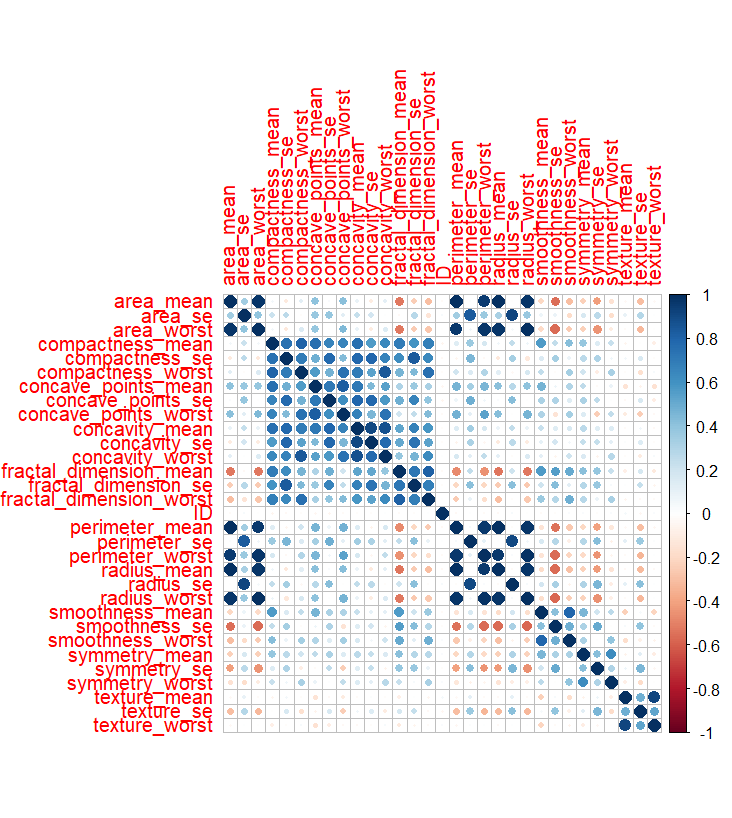
\includegraphics{images/correlation_matrix_benign.png}

\textbf{Correlation Matrix Malignant}:
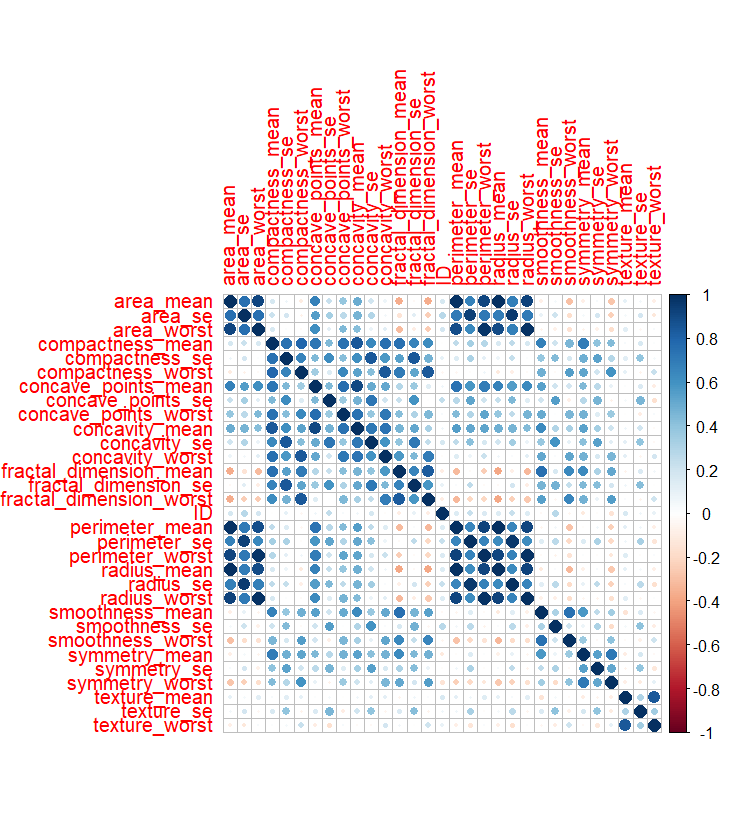
\includegraphics{images/correlation_matrix_malignant.png}

\textbf{Scree Plot}: 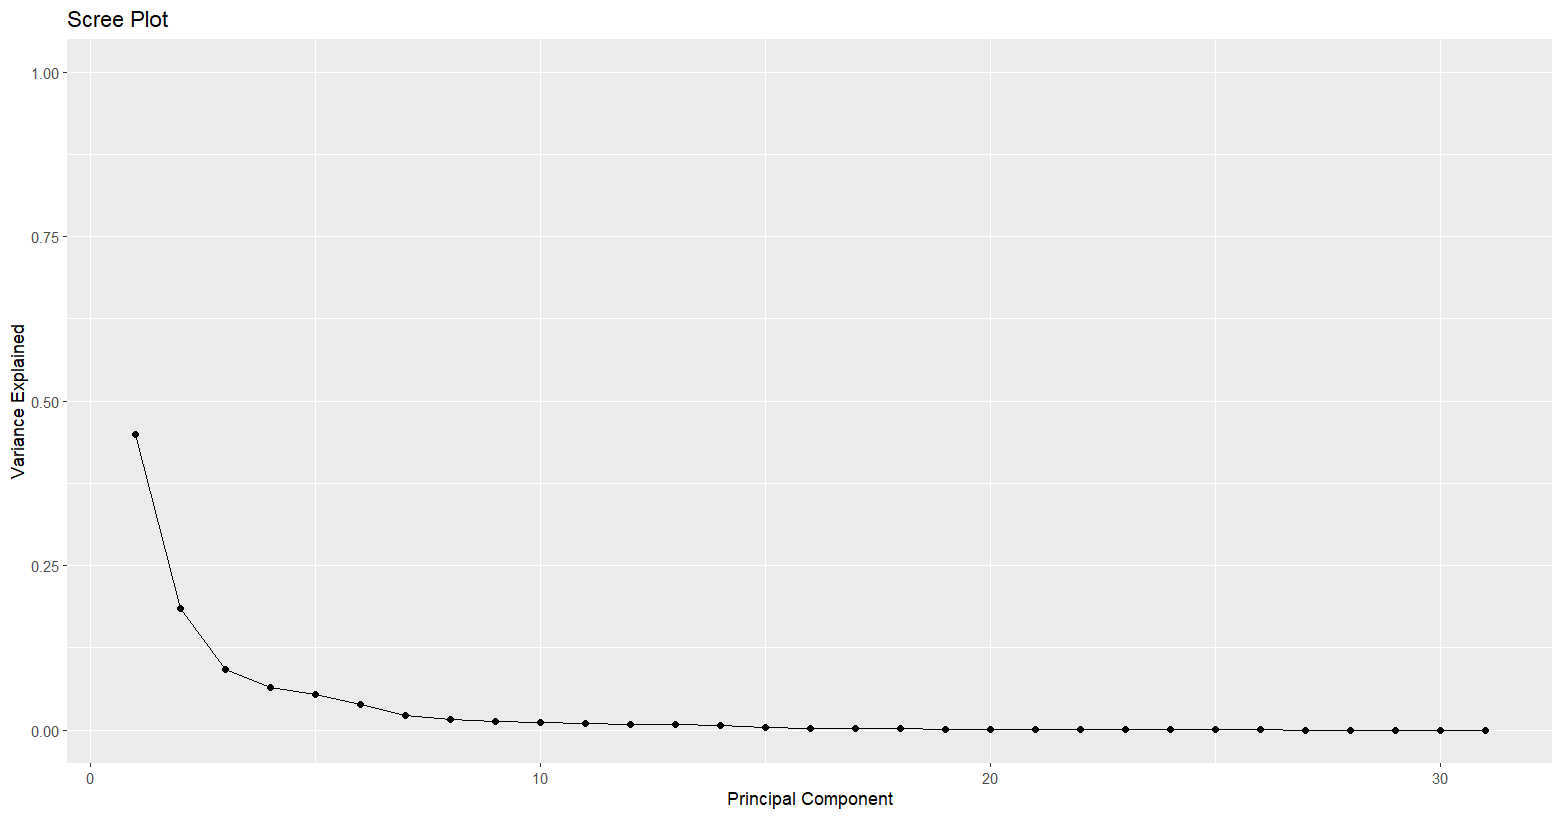
\includegraphics{images/scree_plot_pca.png}

\textbf{T-Distributed\_Stochastic\_Graph}:
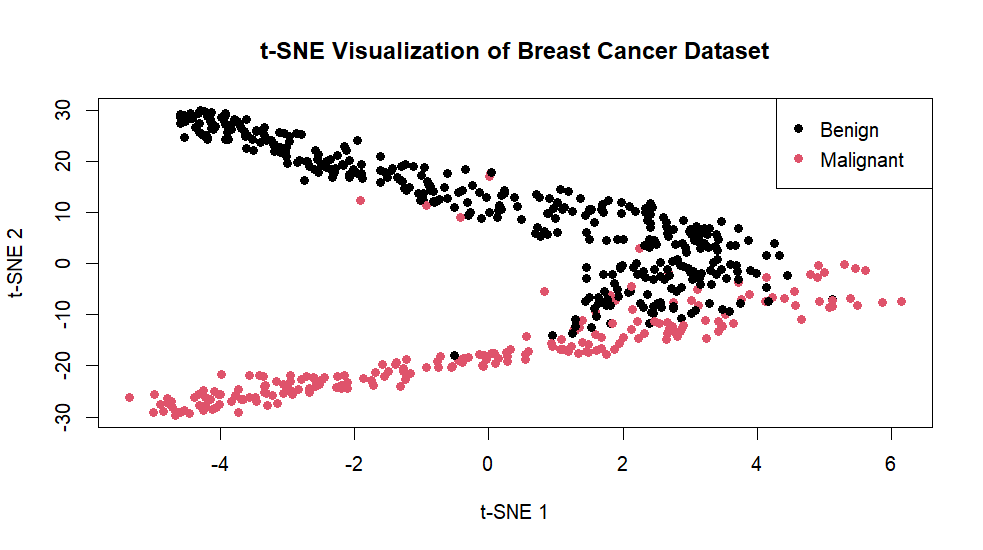
\includegraphics{images/t-distributed_stochastic_graph.png}

\subsection{Conclusion}\label{conclusion}

\begin{itemize}
\tightlist
\item
  \textbf{Takeaways}: In conclusion, the analysis of the correlation
  matrices reveals that variables with the strongest correlations are
  size-based variables. There is some multicollinearity, where plotting
  the same variable against itself results in a correlation of 1.0. LDA
  and QDA were then used to explain the coefficients and group means for
  the purpose of binary classification. Interestingly, QDA slightly
  outperforms LDA, indicating that the original data may not be
  perfectly linear. For further explanation about the variation among
  variables, Principal Component Analysis was employed. The most
  variation was explained in the first and second principal components,
  with a decreasing amount of variation explained by the subsequent
  components. This is further illustrated through the use of the t-SNE
  algorithm, where the model is trained. The purpose of this was to
  illustrate the difference between the first and second principal
  components and convey the difference between benign and malignant
  cases. As shown in the visualisation, there is some overlap between
  benign and malignant cases.
\end{itemize}

\subsection{References}\label{references}

Some of the sources used for reference are from
\href{https://www.statlearning.com/}{An Introduction to Statistical
Learning with Applications in R}. For the particular code used in this
project, please feel free to access the following github repository
\href{https://github.com/NathanielPyle/NathanielPyle.github.io}{Nathaniel
Pyle}.

\subsection{Citation}\label{citation}

The following citation and acknowledgements are made to the original
creators of this dataset.

Dr.~William H. Wolberg, General Surgery Dept., University of Wisconsin,
Clinical Sciences Center, Madison, WI 53792
\href{mailto:wolberg@eagle.surgery.wisc.edu}{\nolinkurl{wolberg@eagle.surgery.wisc.edu}}

W. Nick Street, Computer Sciences Dept., University of Wisconsin, 1210
West Dayton St., Madison, WI 53706
\href{mailto:street@cs.wisc.edu}{\nolinkurl{street@cs.wisc.edu}}
608-262-6619

Olvi L. Mangasarian, Computer Sciences Dept., University of Wisconsin,
1210 West Dayton St., Madison, WI 53706
\href{mailto:olvi@cs.wisc.edu}{\nolinkurl{olvi@cs.wisc.edu}}

rmarkdown::render(``Breast-Cancer-Wisconsin-Dataset.Rmd'')

\end{document}
